\scnstructheader{Описание подсистемы взаимодействия c sc-памятью на основе языка JSON}
\scnstartsubstruct

\scnheader{Реализация подсистемы взаимодействия c sc-памятью на основе языка JSON}
\scnexplanation{Реализация подсистемы взаимодействия c sc-памятью на основе языка JSON позволяет ostis-системам взаимодействовать с системами из внешней среды на основе общепринятого транспортного формата передачи данных JSON и предоставляет API для доступа к sc-памяти платформы интерпретации sc-моделей.}
\scnrelfromlist{используемый язык программирования}{C;C++;Python;TypeScript;CSharp;Java}
\scnrelfromlist{используемый язык}{SC-JSON-код}
\scnrelfrom{архитектура}{Клиент-серверная архитектура}
\scnrelto{реализация}{Подсистема взаимодействия с sc-памятью на основе языка JSON}
\scnaddlevel{1}
\scnidtf{Подсистема взаимодействия с sc-памятью на основе формата JSON}
\scnidtf{Подсистема взаимодействия с sc-памятью на основе транспортного формата передачи данных JSON}
\scnexplanation{Взаимодействие c sc-памятью обеспечивается с помощью передачи информации на \textit{\textbf{SC-JSON-коде}} и ведётся, с одной стороны, между сервером, являющегося частью ostis-системы, написанным на том же языке реализации этой ostis-системы и имеющим доступ к её sc-памяти, и с другой стороны множеством клиентом, которым известно о наличии сервера в пределах сети их использования.}
\scnnote{Языки \textit{\textbf{SC-JSON-код}} и \textit{\textbf{SС-код}} схожи денотационной семантикой, осмысленные фрагменты текстов обоих языков представляют семантически корректную структуру сущностей и связей между ними.}
\scnnote{С помощью подсистемы взаимодействия с sc-памятью на основе языка JSON можно взаимодействовать с ostis-системой на таком же множестве возможных операций, как и в случае, если бы взаимодействие происходило (непосредственно) напрямую, на том же языке реализации платформы интерпретации sc-моделей компьютерных систем. При этом результат работы отличается только скоростью обработки информации.}
\scnsubdividing{
Серверная система на основе Websocket, обеспечивающая доступ к sc-памяти платформы интерпретации sc-моделей при помощи команд SC-JSON-кода\\;
Множество клиентских систем, подключаемых и взаимодействующих с \textit{Серверной системой на основе Websocket, обеспечивающей доступ к sc-памяти платформы интерпретации sc-моделей при помощи команд SC-JSON-кода}\\
\scnaddlevel{1}
\scnsubdividing{
Клиентская система, подключаемая и взаимодействующая с \textit{SC-сервером}, реализованная на языке программирования Python\\;
Клиентская система, подключаемая и взаимодействующая с \textit{SC-сервером}, реализованная на языке программирования TypeScript\\;
Клиентская система, подключаемая и взаимодействующая с \textit{SC-сервером}, реализованная на языке программирования CSharp\\;
Клиентская система, подключаемая и взаимодействующая с \textit{SC-сервером}, реализованная на языке программирования Java\\;
}
\scnaddlevel{-1}
}
\scnaddlevel{-1}

\scnheader{SC-JSON-код}
\scnidtf{Semantic JSON-code}
\scnidtf{Semantic JavaScript Object Notation code}
\scnidtf{Язык внешнего смыслового представления знаний для взаимодействия с ostis-системами на основе языка JSON}
\scnidtf{Метаязык, являющийся подмножеством языка JSON и обеспечивающий внешнее представление и структуризацию \textit{sc-текстов}, используемых ostis-системой в процессе своего функционирования и взаимодействия со внешней средой.}
\scntext{основной внешний идентификатор sc-элемента}{\textbf{SC-JSON-код}}
\scnaddlevel{1}
\scniselement{имя собственное}
\scnaddlevel{-1}
\scntext{часто используемый неосновной внешний идентификатор sc-элемента}{sc-json-текст}
\scnaddlevel{1}
\scniselement{имя нарицательное}
\scnaddlevel{-1}
\scniselement{абстрактный язык}
\scniselement{линейный язык}
\scnsuperset{JSON}
\filemodetrue
\scnrelfromvector{принципы, лежащие в основе}{
Тексты, описываемые на языке внешнего представления знаний \textit{\textbf{SC-JSON-код}} представляют собой линейную структуру, представляемую в виде линейного строкового текста и состоящую из набора корректных осмысленных команд, записанных в виде \textit{sc-json-пар} вида \{отношение: объект\}, где отношением выступает знак квазибинарного отношения, состоящего из пар вида \{субъект: объект\}, где объектом выступает знак, обозначаемый предложением, включающее такие пары, а субъектом - sc-json-объекты: sc-json-литерал, sc-json-списки sc-json-объектов, sc-json-предложения, состоящие из sc-json-списков sc-json-объектов; 
Тексты \textit{\textbf{SC-JSON-кода}} представляют собой sc-json-команды. Каждая команда представляет собой json-объект, в котором указываются уникальный идентификатор команды, тип этой команды и ее аргументы. C каждой командой ассоциируется ответ на эту команду. Ответ на команду представляет собой команду, в котором указываются идентификатор команды, ее статус (выполнена успешно/безуспешно) и результаты. Структура аргументов и результатов команды определяется типом команды. Для каждого ответа существует запрос.}
\filemodefalse 
\scnrelfromlist{достоинство}{
\scnfileitem{Язык JSON является общепринятым открытым форматом, для работы с которым существует большое количество библиотек для популярных языков программирования. Это, в свою очередь, упрощает реализацию клиента и сервера для протокола, построенного на базе \textit{\textbf{SC-JSON-код}}.};
\scnfileitem{Реализация подсистемы взаимодействия со внешней средой на базе \textit{\textbf{SC-JSON-код}} не накладывает принципиальных ограничений на объем (длину) каждой команды, в отличие от других бинарных протоколов. Таким образом, появляется возможность использования неатомарных команд, позволяющих, например, за один акт пересылки такой команды по сети создать сразу несколько sc-элементов. Важными примерами таких команд являются \textit{Команда генерации по произвольному образцу} и \textit{Команда поиска по произвольному образцу}.}}
\scnnote{Можно сказать, что язык на базе JSON является следующим шагом на пути к созданию мощного и универсального языка запросов, аналогичного языку SQL для реляционных баз данных и предназначенному для работы с sc-памятью. Следующий шагом станет реализация такого протокола на основе одного из стандартов внешнего отображения sc-конструкций, например, \textit{SCs-кода}, что, в свою очередь, позволит передавать в качестве команд целые программы обработки sc-конструкций, например на языке SCP.}

\scnstructheader{Синтаксис SC-JSON-кода}
\scnstartsubstruct
\scnheader{Синтаксис SC-JSON-кода}
\scnnote{\textit{Синтаксис SC-JSON-кода} задается: (1) \textit{Алфавитом SC-JSON-кода}, (2) Грамматикой SC-JSON-кода}
\scnrelto{синтаксис}{SC-JSON-код}

\scnheader{Алфавит SC-JSON-кода\scnsupergroupsign}
\scnidtf{Множество всех возможных символов в SC-JSON-коде}
\scnexplanation{Поскольку SC-JSON-код является линейным строковым языком представления знаний, то его алфавит включает объединение алфавитов всех языков, тексты на которых могут представлять внешние идентификаторы и/или содержание sc-ссылок, множество всех цифр и множество всех других специальных символов.}
\scnrelto{алфавит}{SC-JSON-код}

\scnheader{Грамматика SC-JSON-кода}
\scnidtf{Множество всех возможных правил, используемых при построении команд и ответов на них на SC-JSON-коде}
\scnexplanation{Каждой команде \textit{SC-JSON-кода} однозначно соответствует правило грамматики \textit{SC-JSON-кода}.}
\scnrelto{грамматика}{SC-JSON-код}
\scnnote{Правила грамматики \textit{SC-JSON-кода} позволяют определить корректность запрашиваемой команды.}
\scnhaselement{Правило написания \textit{Команды создания sc-элементов}}
\scnaddlevel{1}
\scnrelto{обобщённая структура}{\scnfileimage{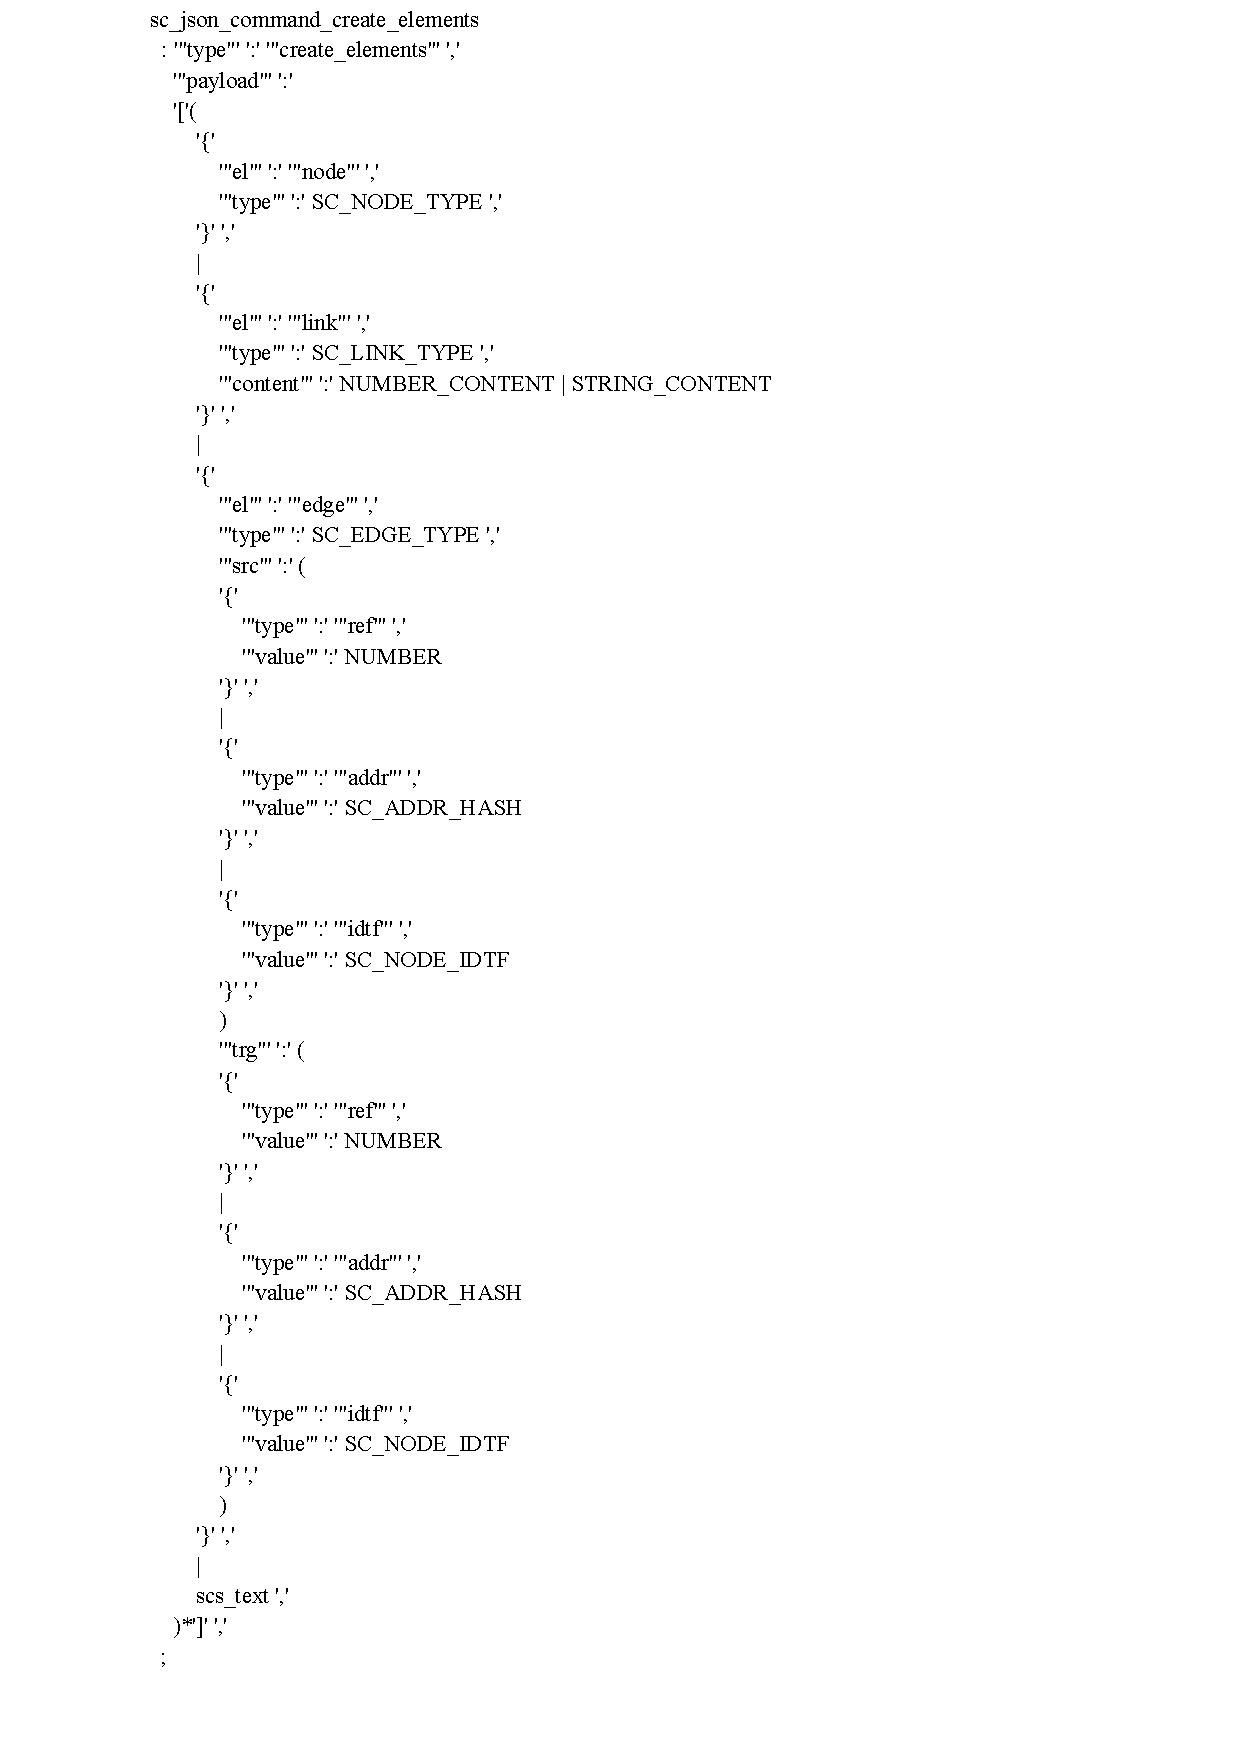
\includegraphics[scale=0.95]{images/create_elements_command}}}
\scnaddlevel{1}
\scnsuperset{Язык описания грамматики языков ANTLR}
\scnrelto{интерпретация}{}
\scnaddlevel{-1}
\scnaddlevel{-1}
\scnhaselement{Правило написания \textit{Команды получения соответствующих типов sc-элементов}}
\scnaddlevel{1}
\scnrelto{обобщённая структура}{\scnfileimage{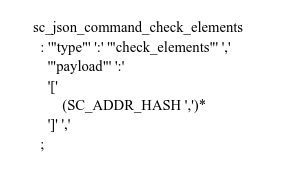
\includegraphics[scale=0.95]{images/check_elements_command}}}
\scnaddlevel{1}
\scnsuperset{Язык описания грамматики языков ANTLR}
\scnrelto{интерпретация}{}
\scnaddlevel{-1}
\scnaddlevel{-1}

\scnendstruct \scninlinesourcecommentpar{Завершили представление \textit{Синтаксиса SC-JSON-кода}}

\scnheader{Серверная система на основе Websocket, обеспечивающая доступ к sc-памяти платформы интерпретации sc-моделей при помощи команд SC-JSON-кода}
\scnidtf{Система, работающая по принципам Websocket и предоставляющая параллельно-асинхронный многоклиентский доступ к sc-памяти платформы интерпретации sc-моделей при помощи SC-JSON-кода}
\scnidtf{SC-JSON-сервер}
\scntext{часто используемый неосновной внешний идентификатор sc-элемента}{SC-сервер}
\scnrelfromlist{используемый язык программирования}{C;C++}
\scnrelfromlist{используемый язык}{SC-JSON-код}
\scnexplanation{Стоит отметить, что текущая реализация \textit{Серверной системы на основе Websocket, обеспечивающая доступ к sc-памяти платформы интерпретации sc-моделей при помощи команд SC-JSON-кода} не является первой в своём роде и заменяет предыдущую её реализацию, написанную на языке Python. Причиной такой замены состоит в следующем:
	\begin{scnitemize}
		\item предыдущая реализация \textit{Серверной системы на основе Websocket, обеспечивающая доступ к sc-памяти платформы интерпретации sc-моделей при помощи команд SC-JSON-кода}, реализованная на языке программирования Python, зависит от библиотеки Boost Python, предоставляемой сообществом по развитию и коллаборации языков С++ и Python. Дело в том, что такое решение требует поддержки механизма интерпретации программного кода на языке Python на язык С++, что является избыточным и необоснованным, поскольку большая часть программного кода \textit{\textbf{Программного варианта реализации платформы интерпретации sc-моделей компьютерных систем}} реализована на языках С и С++. Новая реализация описываемой программной системы позволяет избавиться от использования ёмких библиотек (например, boost-python-lib, llvm) и языка Python;
		\item при реализации распределённых подсистем важную роль играет скорость обработки знаний, то есть возможность быстро и срочно отвечать на запросы пользователя. Качество доступа к sc-памяти посредством реализованной \textit{Подсистемы взаимодействия с sc-памятью на основе языка JSON} должно быть соизмеримо с качеством доступа к sc-памяти при помощи специализированного программного интерфейса API, реализованного на том же языке программирования, что и сама система. С этой точки зрения скорость обработки запросов \textit{Подсистемой взаимодействия с sc-памятью на основе языка JSON}, в том числе и обработка знаний, повышена не менее чем в 1,5 раза по сравнению с предыдущим вариантом реализации этой подсистемы.
	\end{scnitemize}
}

\bigskip
\scnendstruct \scninlinesourcecommentpar{Завершили описание \textit{Подсистемы взаимодействия c sc-памятью на основе языка JSON}}